\let\negmedspace\undefined
\let\negthickspace\undefined
\documentclass[journal,12pt,twocolumn]{IEEEtran}
%\documentclass[conference]{IEEEtran}
%\IEEEoverridecommandlockouts
% The preceding line is only needed to identify funding in the first footnote. If that is unneeded, please comment it out.
\usepackage{svg}
\usepackage{tikz, pgfplots}
\usepackage{cite}
\usepackage{amsmath,amssymb,amsfonts,amsthm}
\usepackage{algorithmic}
\usepackage{graphicx,wrapfig}
\usepackage{textcomp}
\usepackage{xcolor}
\usepackage{txfonts}
\usepackage{listings}
\usepackage{enumitem}
\usepackage{mathtools}
\usepackage{gensymb}
\usepackage[breaklinks=true]{hyperref}
\usepackage{tkz-euclide} % loads  TikZ and tkz-base
\usepackage{listings}


\usetikzlibrary{positioning}
%
%\usepackage{setspace}
%\usepackage{gensymb}
%\doublespacing
%\singlespacing

%\usepackage{graphicx}
%\usepackage{amssymb}
%\usepackage{relsize}
%\usepackage[cmex10]{amsmath}
%\usepackage{amsthm}
%\interdisplaylinepenalty=2500
%\savesymbol{iint}
%\usepackage{txfonts}
%\restoresymbol{TXF}{iint}
%\usepackage{wasysym}
%\usepackage{amsthm}
%\usepackage{iithtlc}
%\usepackage{mathrsfs}
%\usepackage{txfonts}
%\usepackage{stfloats}
%\usepackage{bm}
%\usepackage{cite}
%\usepackage{cases}
%\usepackage{subfig}
%\usepackage{xtab}
%\usepackage{longtable} 
%\usepackage{multirow}
%\usepackage{algorithm}
%\usepackage{algpseudocode}
%\usepackage{enumitem}
%\usepackage{mathtools}
%\usepackage{tikz}
%\usepackage{circuitikz}
%\usepackage{verbatim}
%\usepackage{tfrupee}
%\usepackage{stmaryrd}
%\usetkzobj{all}
%    \usepackage{color}                                            %%
%    \usepackage{array}                                            %%
%    \usepackage{longtable}                                        %%
%    \usepackage{calc}                                             %%
%    \usepackage{multirow}                                         %%
%    \usepackage{hhline}                                           %%
%    \usepackage{ifthen}                                           %%
  %optionally (for landscape tables embedded in another document): %%
%    \usepackage{lscape}     
%\usepackage{multicol}
%\usepackage{chngcntr}
%\usepackage{enumerate}

%\usepackage{wasysym}
%\newcounter{MYtempeqncnt}
\DeclareMathOperator*{\Res}{Res}
%\renewcommand{\baselinestretch}{2}
\renewcommand\thesection{\arabic{section}}
\renewcommand\thesubsection{\thesection.\arabic{subsection}}
\renewcommand\thesubsubsection{\thesubsection.\arabic{subsubsection}}

\renewcommand\thesectiondis{\arabic{section}}
\renewcommand\thesubsectiondis{\thesectiondis.\arabic{subsection}}
\renewcommand\thesubsubsectiondis{\thesubsectiondis.\arabic{subsubsection}}

% correct bad hyphenation here
\hyphenation{op-tical net-works semi-conduc-tor}
\def\inputGnumericTable{}                                 %%

\lstset{
%language=C,
frame=single, 
breaklines=true,
columns=fullflexible
}
%\lstset{
%language=tex,
%frame=single, 
%breaklines=true
%}

\begin{document}
%


\newtheorem{theorem}{Theorem}[section]
\newtheorem{problem}{Problem}
\newtheorem{proposition}{Proposition}[section]
\newtheorem{lemma}{Lemma}[section]
\newtheorem{corollary}[theorem]{Corollary}
\newtheorem{example}{Example}[section]
\newtheorem{definition}[problem]{Definition}
%\newtheorem{thm}{Theorem}[section] 
%\newtheorem{defn}[thm]{Definition}
%\newtheorem{algorithm}{Algorithm}[section]
%\newtheorem{cor}{Corollary}
\newcommand{\BEQA}{\begin{eqnarray}}
\newcommand{\EEQA}{\end{eqnarray}}
\newcommand{\define}{\stackrel{\triangle}{=}}
\newcommand\tab[1][1cm]{\hspace*{#1}}
\bibliographystyle{IEEEtran}
%\bibliographystyle{ieeetr}


\providecommand{\mbf}{\mathbf}
\providecommand{\pr}[1]{\ensuremath{\Pr\left(#1\right)}}
% Added from https://raw.githubusercontent.com/gadepall/digital-communication/main/probability/trans.tex %%
\newcommand*{\permcomb}[4][0mu]{{{}^{#3}\mkern#1#2_{#4}}}
\newcommand*{\perm}[1][-3mu]{\permcomb[#1]{P}}
\newcommand*{\comb}[1][-1mu]{\permcomb[#1]{C}}
\providecommand{\gauss}[2]{\mathcal{N}
\ensuremath{\left(#1,#2\right)}}
%%
\providecommand{\qfunc}[1]{\ensuremath{Q\left(#1\right)}}
\providecommand{\sbrak}[1]{\ensuremath{{}\left[#1\right]}}
\providecommand{\lsbrak}[1]{\ensuremath{{}\left[#1\right.}}
\providecommand{\rsbrak}[1]{\ensuremath{{}\left.#1\right]}}
\providecommand{\brak}[1]{\ensuremath{\left(#1\right)}}
\providecommand{\lbrak}[1]{\ensuremath{\left(#1\right.}}
\providecommand{\rbrak}[1]{\ensuremath{\left.#1\right)}}
\providecommand{\cbrak}[1]{\ensuremath{\left\{#1\right\}}}
\providecommand{\lcbrak}[1]{\ensuremath{\left\{#1\right.}}
\providecommand{\rcbrak}[1]{\ensuremath{\left.#1\right\}}}
\theoremstyle{remark}
\newtheorem{rem}{Remark}
\newcommand{\sgn}{\mathop{\mathrm{sgn}}}
\providecommand{\abs}[1]{\(left\)vert#1\(right\)vert}
\providecommand{\res}[1]{\Res\displaylimits_{#1}}
\providecommand{\norm}[1]{\(left\)lVert#1\(right\)rVert}
%\providecommand{\norm}[1]{\lVert#1\rVert}
\providecommand{\mtx}[1]{\mathbf{#1}}
\providecommand{\mean}[1]{E\(left\)[ #1 \(right\)]}
\providecommand{\fourier}{\overset{\mathcal{F}}{ \rightleftharpoons}}
%\providecommand{\hilbert}{\overset{\mathcal{H}}{ \rightleftharpoons}}
\providecommand{\system}{\overset{\mathcal{H}}{ \longleftrightarrow}}
%\newcommand{\solution}[2]{\textbf{Solution:}{#1}}
\newcommand{\solution}{\noindent \textbf{Solution: }}
\newcommand{\cosec}{\,\text{cosec}\,}
\providecommand{\dec}[2]{\ensuremath{\overset{#1}{\underset{#2}{\gtrless}}}}
\newcommand{\myvec}[1]{\ensuremath{\begin{pmatrix}#1\end{pmatrix}}}
\newcommand{\mydet}[1]{\ensuremath{\begin{vmatrix}#1\end{vmatrix}}}

\let\vec\mathbf

\vspace{3cm}

\title{
\textbf {Hardware Assignment}\\ \large \textbf{AI1110}: Probability and Random Variables\\Indian Institute of Technology, Hyderabad
}
\author{Gunethra Bommineni$^{*}$% <-this % stops a space
	% \thanks{*The student is with the Department
		% of Electrical Engineering, Indian Institute of Technology, Hyderabad
		% 502285 India e-mail: ee22btech11205@iith.ac.in.}
  }

\maketitle

\newpage

\bigskip
\renewcommand{\thefigure}{\theenumi}
\renewcommand{\thetable}{\theenumi}

\begin{abstract}
    \textbf{Random Number Generation using Shift Registers}
\end{abstract}

% \section*{Aim:}
% To create a circuit which randomly chooses a hexadecimal number and displays it on a 7-segment display using shift registers.

\section*{Components used:}
\begin{table}[h]
	%%%%%%%%%%%%%%%%%%%%%%%%%%%%%%%%%%%%%%%%%%%%%%%%%%%%%%%%%%%%%%%%%%%%%%
%%                                                                  %%
%%  This is a LaTeX2e table fragment exported from Gnumeric.        %%
%%                                                                  %%
%%%%%%%%%%%%%%%%%%%%%%%%%%%%%%%%%%%%%%%%%%%%%%%%%%%%%%%%%%%%%%%%%%%%%%
\begin{tabular}{|l|c|c|}\hline
	Component &Value &Quantity\\ \hline
    Timer & 555 IC &1 \\ \hline
    X-OR Gate &7486 &1 \\ \hline
    Decoder &7447 &1 \\ \hline
    Flip Flop &7474 &2 \\ \hline
    Capacitor &47 nF &1 \\ \hline
    Capacitor &470 nF &1 \\ \hline
    Resistor &1 K$\Omega$ &1 \\ \hline
    Resistor &10 $M\Omega$ &1 \\ \hline
    7-Segment Display &Common Anode &1 \\ \hline
	Breadboard &840 pins &1 \\ \hline
	Wires & &20 \\ \hline
\end{tabular}
	\caption{Components used}
\end{table}

\section*{Procedure:}
\begin{enumerate}
    % \begin{figure}[h]
    \item We first connect the Timer-555 IC as shown in figure to generate the clock.\ref{555}
    \begin{figure}[h]
		\includegraphics[width=\columnwidth]{figs/555.png}
		\caption{Connecting the Timer-555 IC}
		\label{555}
	\end{figure}

	\item We then connect this clock output to the clock signal of D-Flip flops.

	% \item Then we connected Clock output of 555 timer circuit to the clock signal of D-Flip flops

    % \begin{figure}[h]
	\item Next we make the circuit for shift registers using a 4 D-Flip flops (using the two 7474 IC's) and an XOR gate (7486 IC) according to the figure \ref{Circuit} 
	\begin{figure}[h]
		\includegraphics[width=\columnwidth]{figs/IC7474.png}
		\caption{Pin out for IC 7474}
		\label{7474_IC}
		\includegraphics[width=\columnwidth]{figs/circuit_connections.jpg}
		\caption{Circuit diagram}
		\label{Circuit}
	\end{figure}

    % \begin{figure}[h]
	\item Then we connect the output of each D-Flip Flop ($Q_0$,$Q_1$,$Q_2$,$Q_3$) to the Decoder (7447 IC) (A,B,C,D) respectively as per the figure\ref{7447}
	\begin{figure}[h]
		\includegraphics[width=\columnwidth]{figs/7447.png}
		\caption{Pin out for Decoder gate IC 7447}
		\label{7447}
	\end{figure}

    % \begin{figure}[h]
	\item Next we connect the 7-segment display and connect it with the decoder (7447 IC) according to the table \ref{7447_table} and the figure \ref{Display}
	\begin{figure}[h]
		\includegraphics[scale = 0.2]{figs/7447_disp.png}
		\caption{Connection of seven segmented display with decoder}
		\label{7447_table}
	% \end{figure}
	% \begin{figure}
		\input{figs/tikz}
        \caption{7-segment display}
		\label{Display}
	\end{figure}

	\item Finally we connect all independent parts with each other and then turned on the power source.

\section*{Output} 
	Output was changing digits on the seven segment display the output is shown in figure \ref{output}
	\begin{figure}
		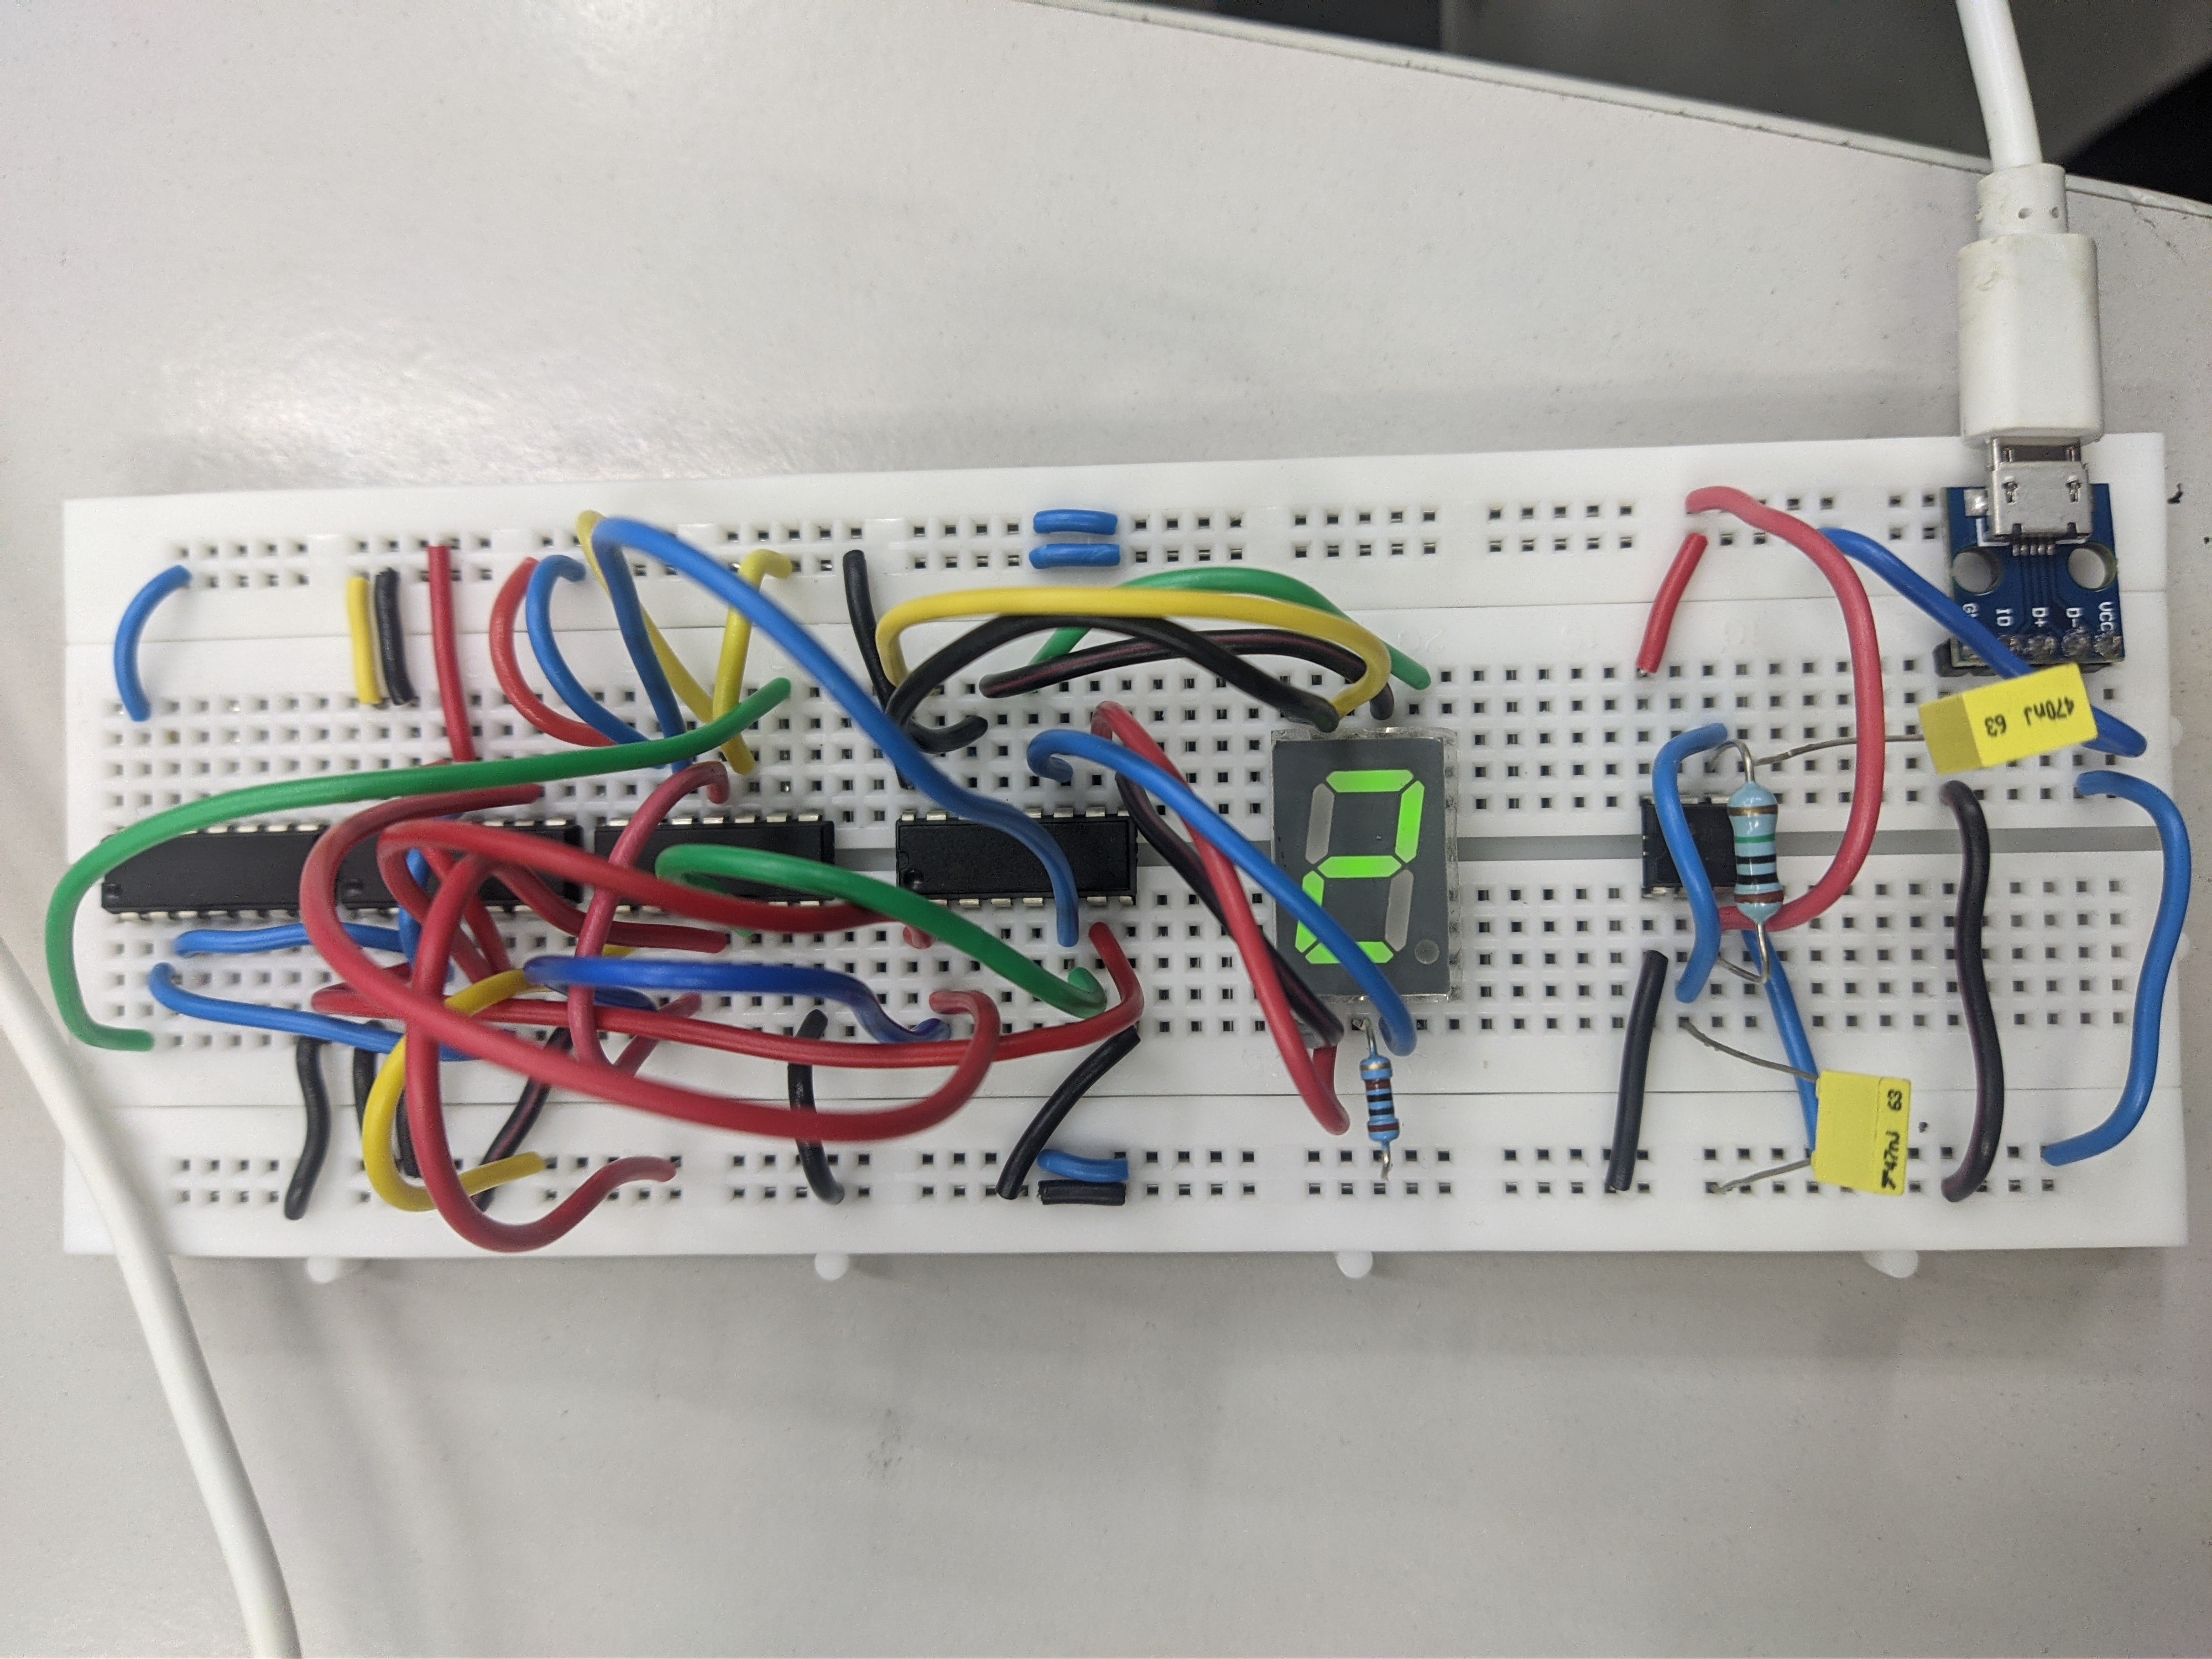
\includegraphics[scale = 0.05]{output/output_1.jpg}
        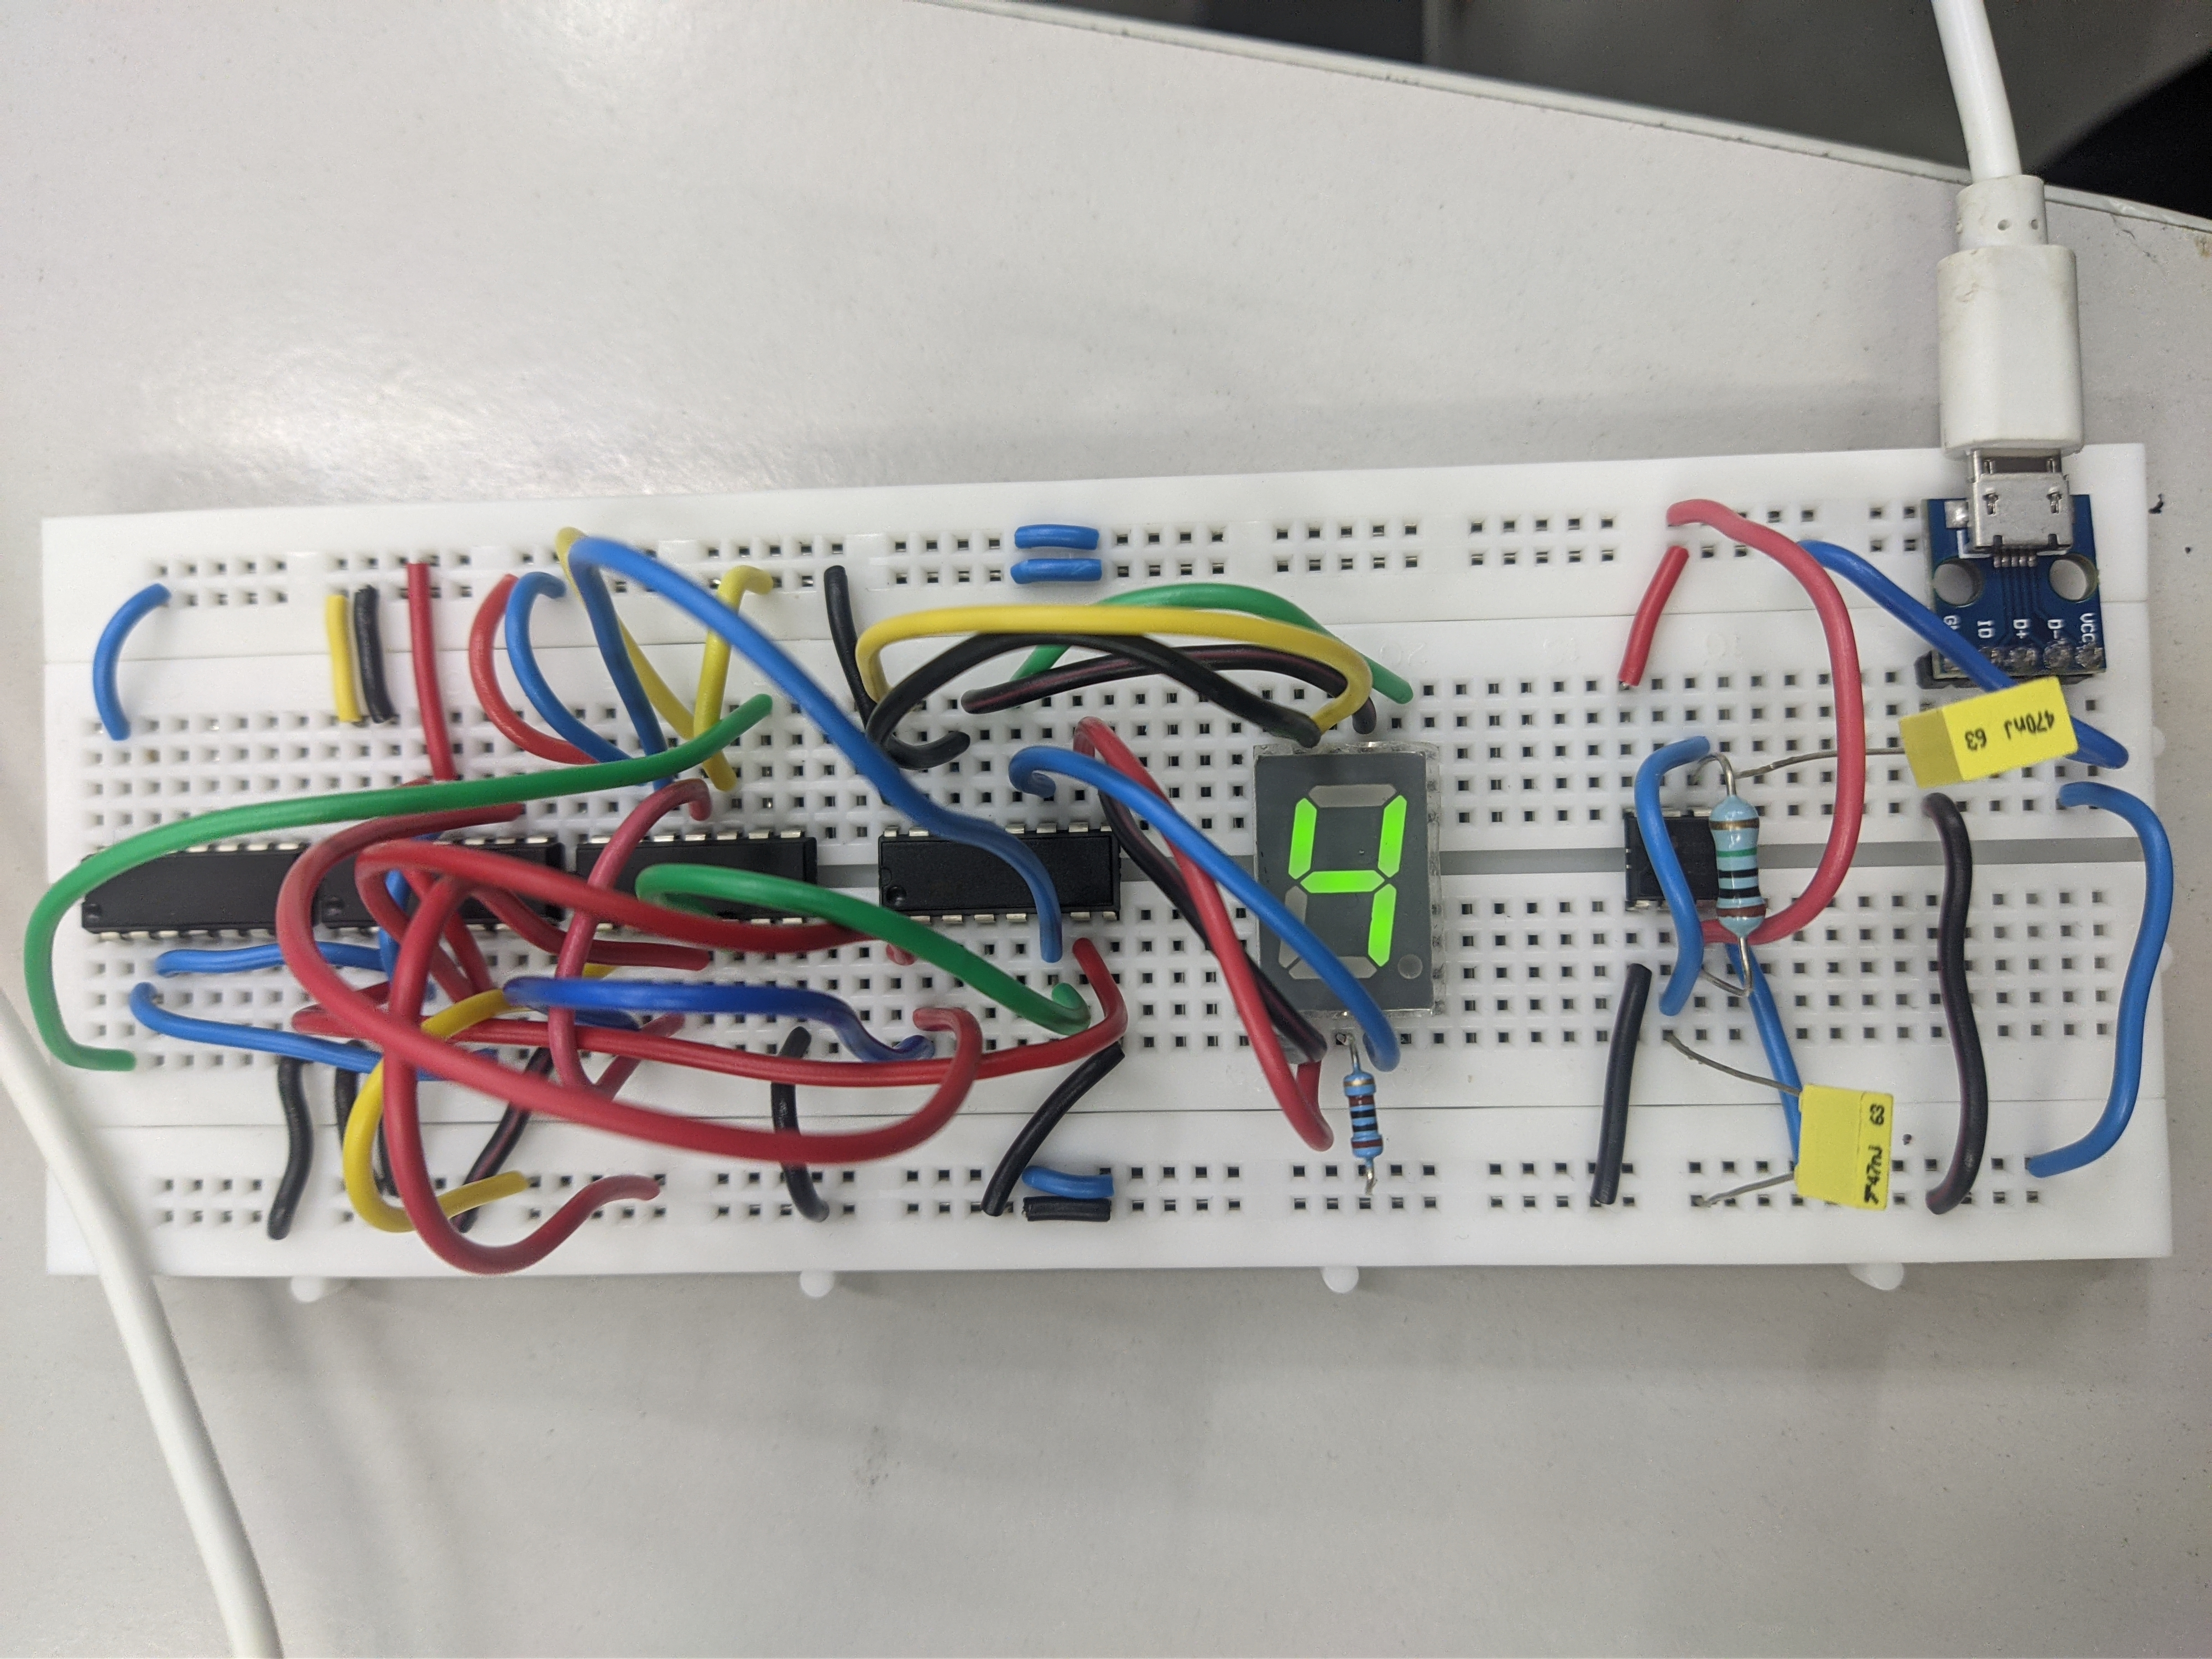
\includegraphics[scale = 0.05]{output/output_2.jpg}
        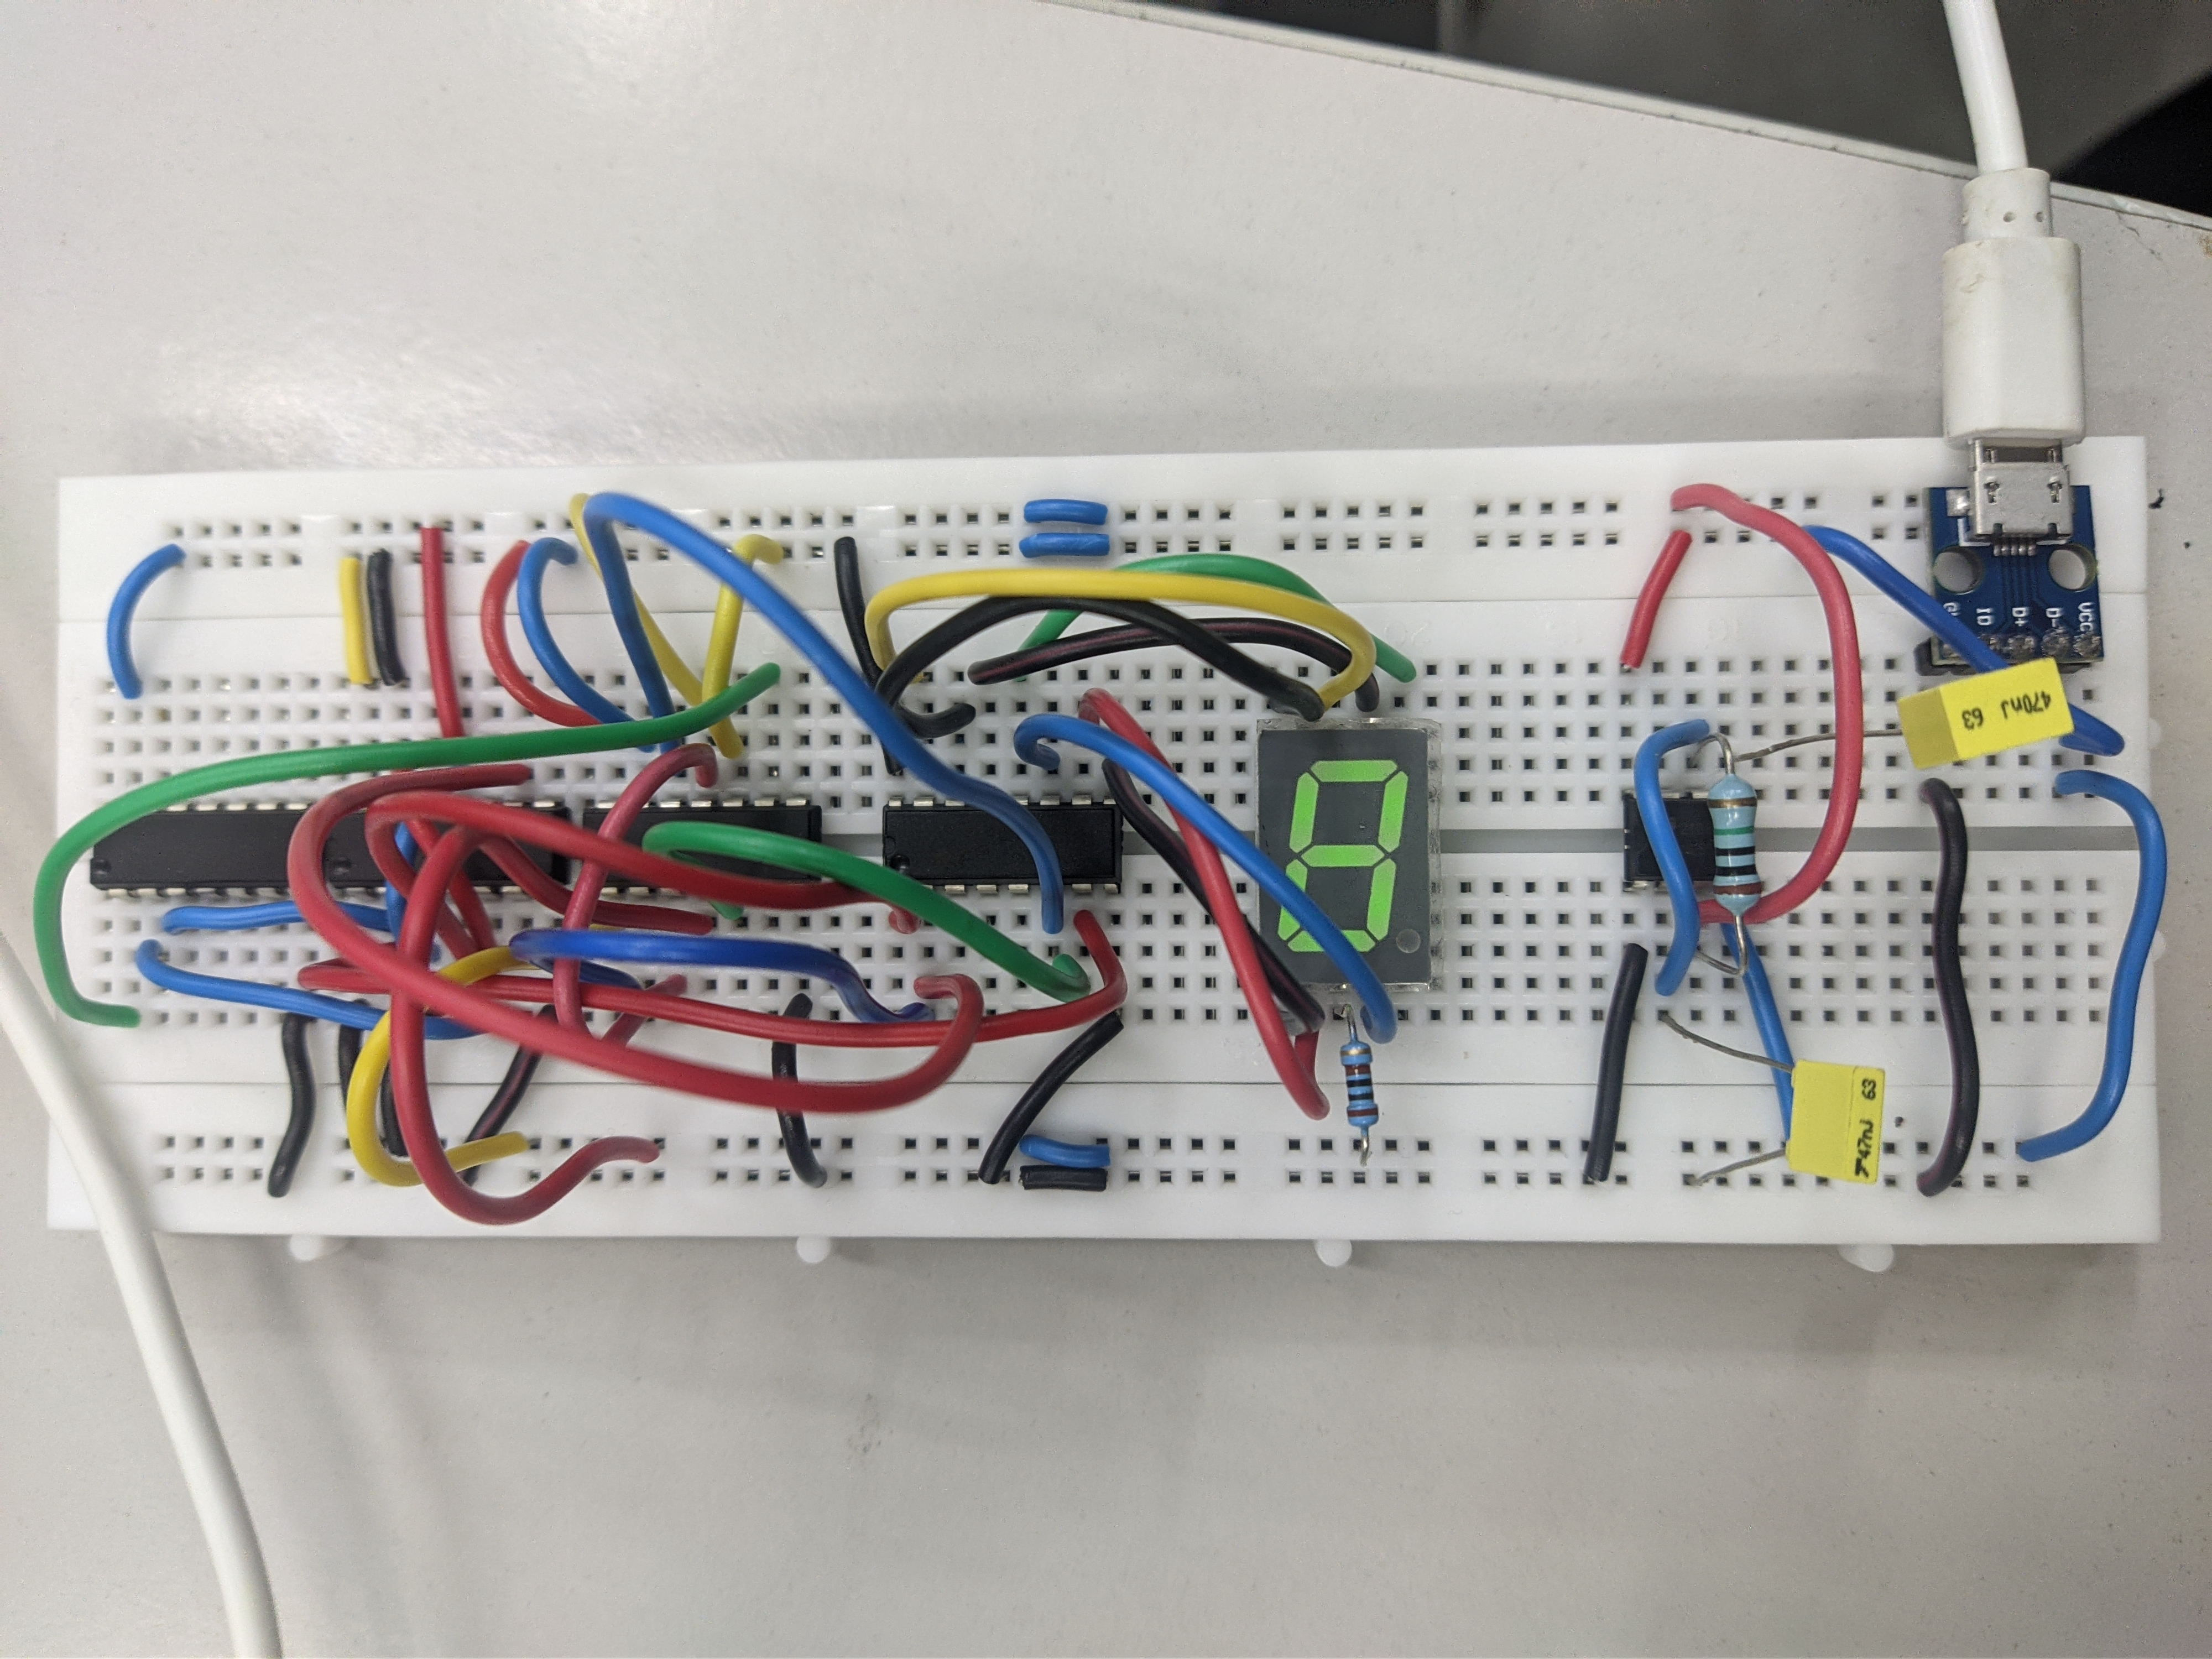
\includegraphics[scale = 0.05]{output/output_3.jpg}
        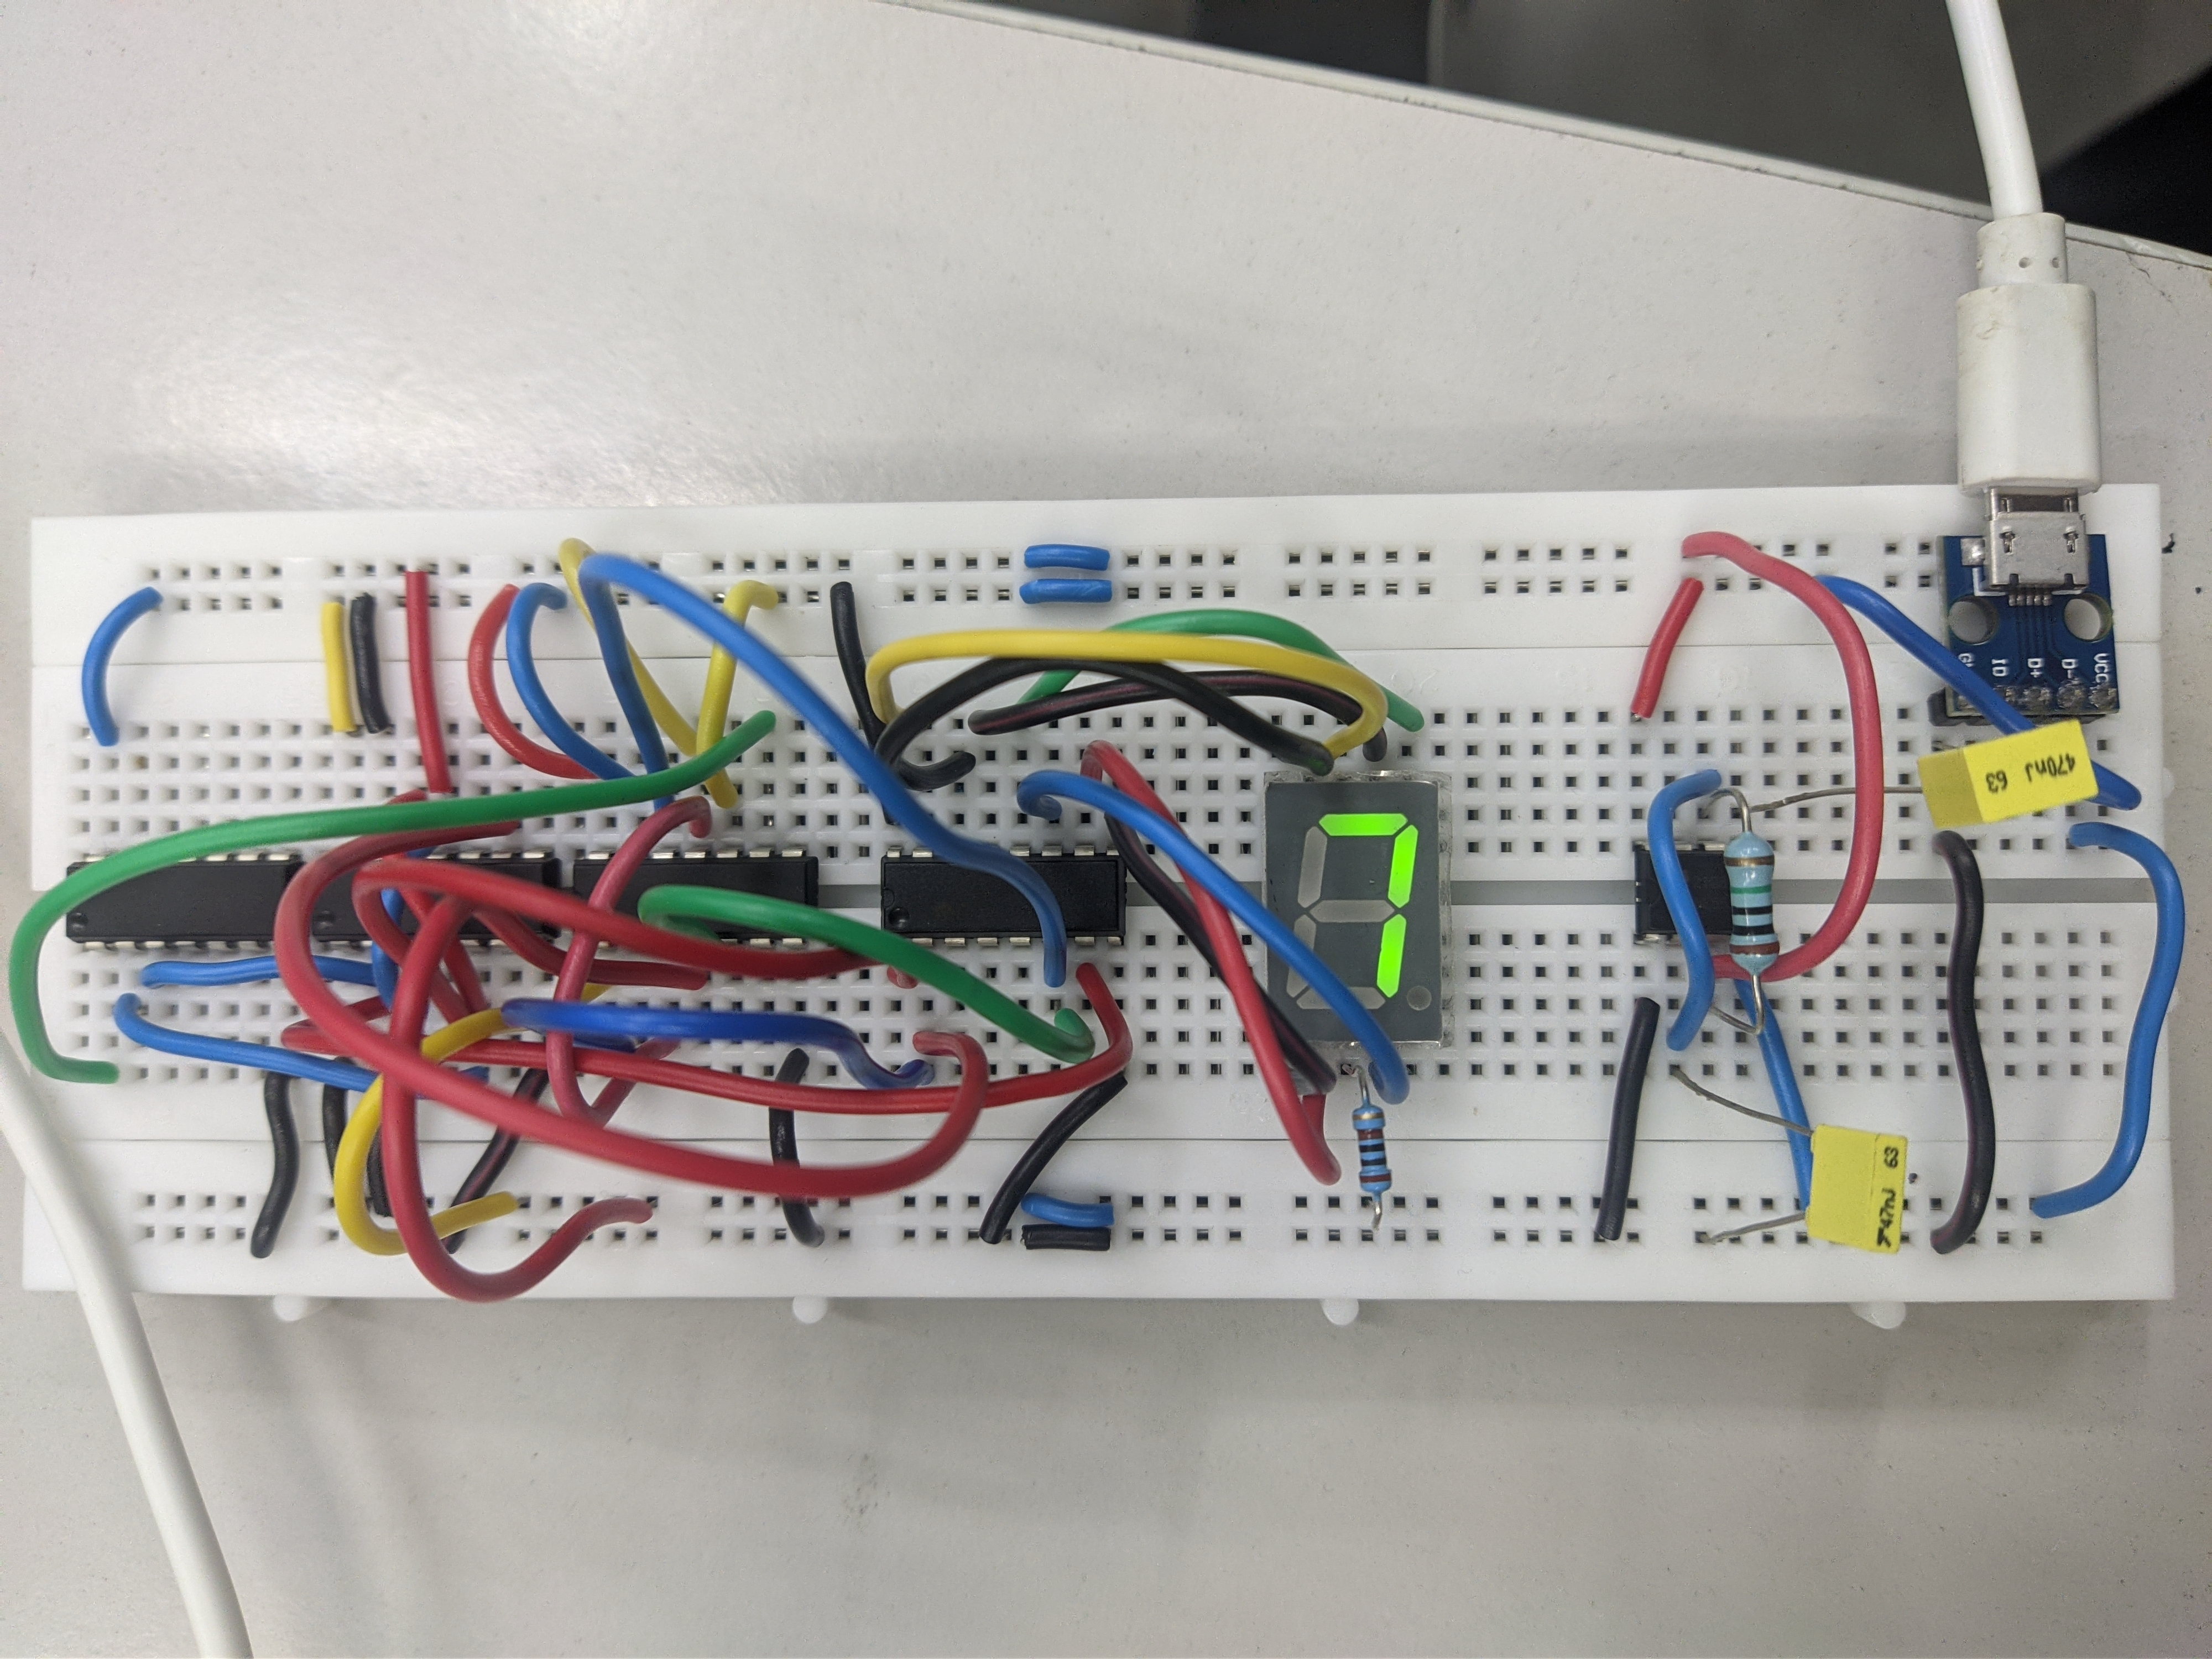
\includegraphics[scale = 0.05]{output/output_4.jpg}
		\caption{Randomizer Output}
		\label{output}
	\end{figure}
	
\end{enumerate}
\end{document}
